\documentclass{article}
    \usepackage[utf8]{inputenc}
    
    \title{关于开Spatial}
    \author{Tian Zhao}
    \date{November 2018}
    
    \usepackage{natbib}
    \usepackage{graphicx}
    \usepackage{xcolor}
    \usepackage{listings}
    \lstset{basicstyle=\ttfamily,
      showstringspaces=false,
      commentstyle=\color{red},
      keywordstyle=\color{blue}
    }
    
    
    \begin{document}
    
    \maketitle
    
    \section{Introduction}
    This document provides a guideline on implementing the Fringe module for Intel Arria10 boards.
    However, this guideline can be generalized to other FPGA platforms as well.
    
    \section{Environment Variables}
    This section includes specifications for environment variables being used in this documentation.
    \begin{itemize}
        \item $Spatial$: The spatial language.
        \item $SPATIAL\_HOME$: The home directory of your installed Spatial.
        \item $JAVA\_HOME$: The home directory of your installed Java.
        \item $IP\_SRC\_HOME$: The directory for storing source files of the $Accel$ IP block.
        \item $FRINGE\_MEM\_BASEADDR$: The base address for shared DRAM between $Host$ and $Accel$.
        \item $FRINGE\_SCALAR\_BASEADDR$: The base address for shared registerfile between $Host$ and $Accel$.
        \item $Accel$: The accelerator hardware. In this document, the accelerator is the targeted Intel Arria 10 board.
        \item $Host$: The host CPU.
        \item $ArgIn$: The Spatial argument registers. This type of registers transfers scalars from $Host$ to $Accel$.
        \item $ArgOut$: The Spatial argument registers. This type of registers transfers scalars from $Accel$ to $Host$.
        \item $DRAM$: The Spatial DRAMs. DRAMs can transfer data bidirectionally between $Host$ and $Accel$.
    \end{itemize}
    
    \section{Spatial App Setup}
    We use $Lab1Part1RegExampleExample$ as the driving application in this document.
    The $Spatial$ implementation can be found in Figure \ref{fig:arginout}.
    The code block between line 11 to 17 creates two $ArgIn$ registers and write two scalar values into them.
    The code block between line 19 to 23 executes $Accel$ and writes the result to an $ArgOut$.
    Line 25 fetches the result at $Host$.
    
    \begin{figure}
    \centering
    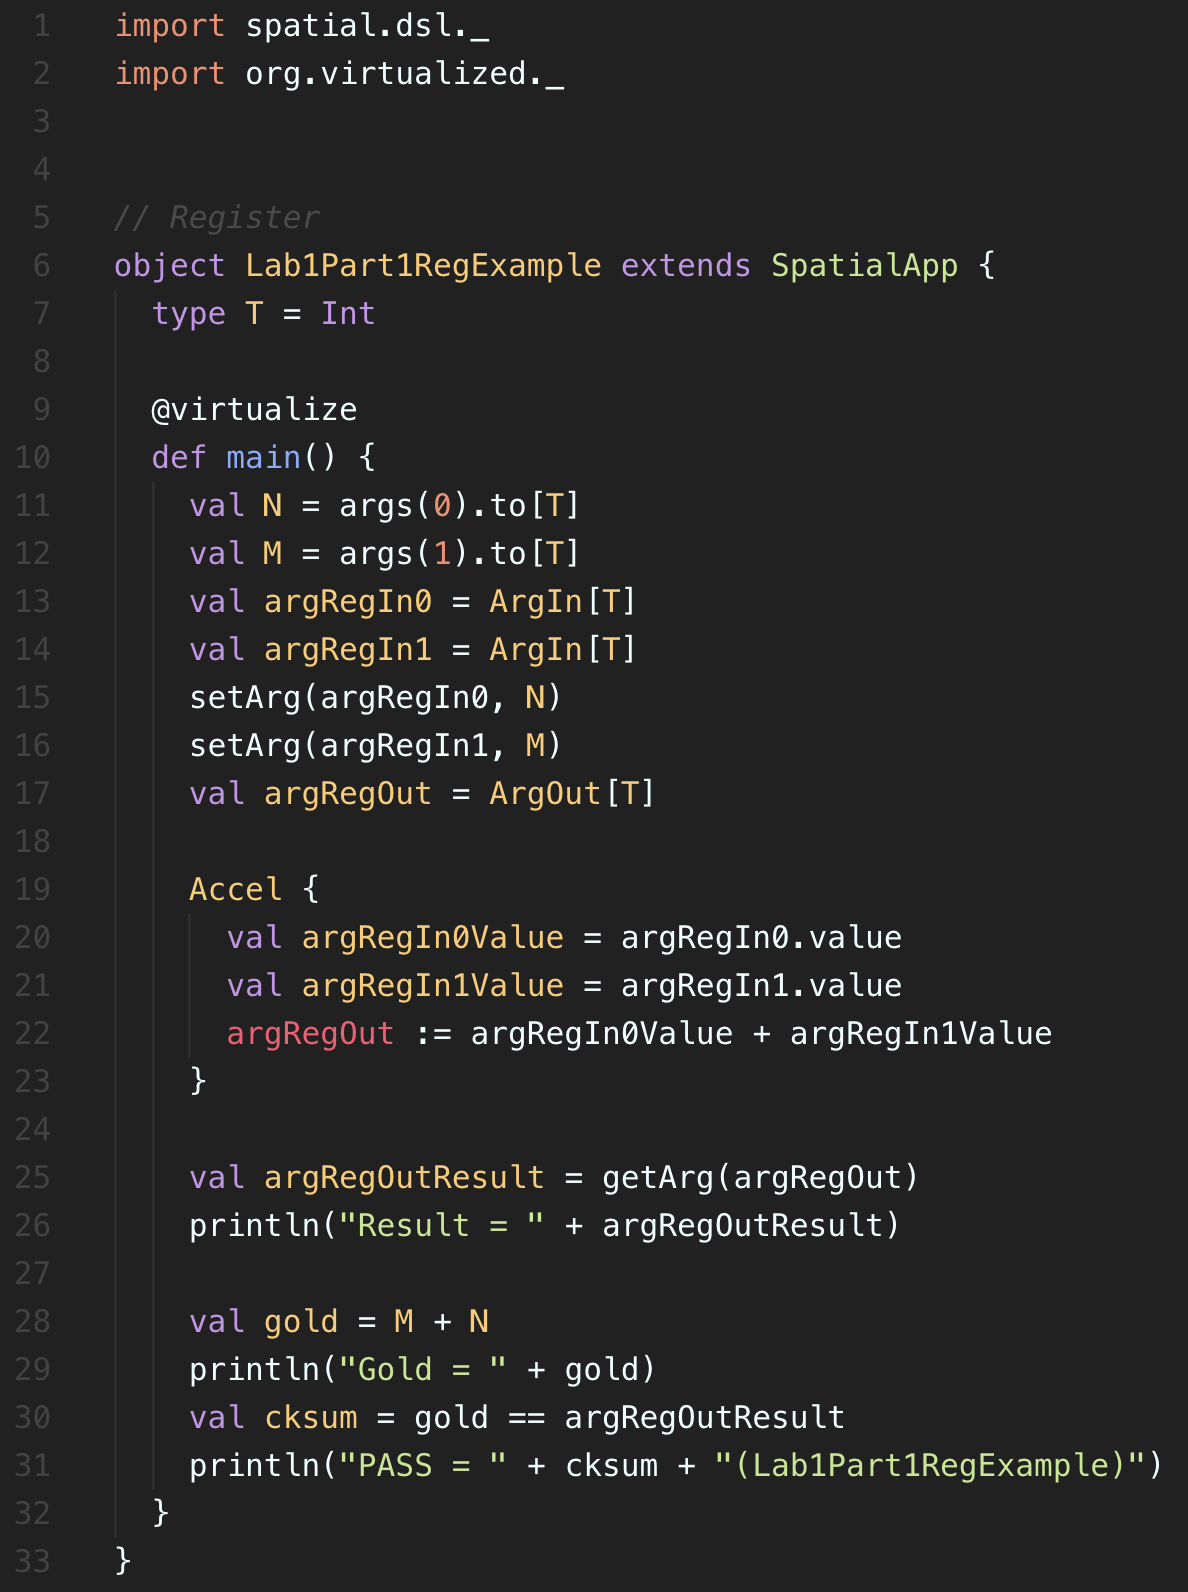
\includegraphics[scale=0.6]{regexample.png}
    \caption{Lab1Part1RegExample. This application performs reading and writing $ArgIn, ArgOut$ registers}
    \label{fig:arginout}
    \end{figure}
    
    \section{Interface between $Host$ and $Accel$}
    $Accel$ and $Host$ share a memory-mapped register file and a DRAM.
    The register file is used for storing $ArgIn$ and $ArgOut$ registers.
    $Accel$ can access this register file using the Avalon-MM lite interface.
    $Host$ can access this register file by memory-mapping it into $Host$'s Virtual Memory Space.
    The DRAM is used for transferring data stored in $DRAM$ objects.
    $Accel$ can access this DRAM using the AXI4-MM interface.
    $Host$ can access this DRAM by memory-mapping it into $Host$'s Virtual Memory Space.
    
    \subsection{Generating $Accel$ Code from $Spatial$}
    A $Spatial$ design can be translated into a $Verilog$ design.
    The Top level of this design is exposed in the form of an AXI4 master interface and an Avalon lite slave interface.
    The following commands will generate the $Verilog$ design for $Lab1Part1RegExample$.
    \begin{lstlisting}[language=bash]
    cd $SPATIAL_HOME
    sbt -batch "apps/run-main Lab1Part1RegExample --synth"
    cd gen/Lab1Part1RegExample
    sbt "runMain top.Instantiator --verilog --testArgs arria10"
    \end{lstlisting}
    
    We can find the generated $Verilog$ design by going to:
    \begin{lstlisting}[language=bash]
    cd $SPATIAL_HOME/gen/Lab1Part1RegExample/verilog-arria10
    \end{lstlisting}
    
    The $Top.v$ file includes the generated design.
    Notice that $SRFF$ is a reserved keyword in Intel's toolchain.
    To avoid naming conflicts, we need to change the name to $SRFF\_sp$:
    \begin{lstlisting}[language=bash]
    sed -i 's/SRFF/SRFF_sp/g' Top.v
    \end{lstlisting}
    
    Now we have the generated design of $Lab1Part1RegExample$ in $Top.v$.
    Next, we need to integrate it into the rest of the system.
    We wrap the design file, $Top.v$, as an IP in Intel's Platform Designer.
    The Platform Designer will handle the process of creating interconnects.
    The next session gives an example on how to create such IP.
    
    \subsection{Creating an IP for $Accel$}
    In this section, we demonstrate the process of wrapping the generated $Verilog$ design
        in an IP and export it to Intel's Platform Designer.
    In the starter project, we provide a folder called $ip\_src$ and a $tcl$ script called $Top\_hw.tcl$.
    $ip\_src$ contains source files for building this IP.
    $Top\_hw.tcl$ specifies the interfaces to communicate with this IP.
    Specifically, the exposed interfaces are Avalon-MM slave and AXI4-MM master.
    You can find more information about these interfaces in the $tcl$ script.
    
    After generating $Top.v$, you can copy it into $ip\_src$.
    Now you can import $Accel$ as an IP in your $Quartus$ project.
    \begin{lstlisting}[language=bash]
    cp Top.v $IP_SRC_HOME/ip_src/
    \end{lstlisting}
    
    A little more information is needed for the $Host$ software.
    When instantiating the $Accel$ IP in your design,
    the Platform Designer will ask for the base addresses of the Avalon-MM and the AX44-MM interfaces.
    These base addresses will be used by the $Host$ code for reading and writing the register files and the memory-mapped DRAM.
    For convenience, we assume that the base address of Avalon-MM is at $FRINGE\_SCALAR\_BASEADDR$,
    and the base address of AXI4-MM is at $FRINGE\_MEM\_BASEADDR$.
    
    \section{Supporting $Host$ Code of $Spatial$}
    In this tutorial, we assume that the $Host$ uses $ARM$ compilers.
    If you are using a different compiler for $cpp$, you can change the compiler options in
    $\$SPATIAL\_HOME/gen/Lab1Part1RegExample/scripts/arria10.mk$.
    
    \subsection{$Host$ API Specifications}
    First, move into the $Host$ code directory by running:
    \begin{lstlisting}[language=bash]
    cd $SPATIAL_HOME/gen/Lab1Part1RegExample/cpp/
    \end{lstlisting}
    
    The logic for running $Accel$ is autogenerated by $Spatial$ and is stored in $TopHost.cpp$.
    $TopHost.cpp$ first loads the bitstream to $Accel$ using $load$ function.
    Then, it sets the $ArgIn$, $ArgOut$ registers using $setArg$ functions.
    If your design contains $DRAM$,  $TopHost$ will also set addresses for the $DRAM$ using $setArg$ functions.
    To move data from $Host$ to $Accel$, $TopHost$ will call $memcpy$.
    After the setup is done, $TopHost$ calls $run$ to start $Accel$.
    Once $Accel$ finishes, $TopHost$ will call $getArg$ to collect the final results.
    If your design contains $DRAM$, $TopHost$ will call $memcpy$ to copy data from $Accel$ to $Host$.
    $setArg$ and $getArg$ functions are implemented using $readReg$ and $writeReg$ functions.
    $run$ function is implemented using $setArg$, $getArg$.
    
    We can see that $load$, $readReg$, $writeReg$, $memcpy$ are the key functions for $TopHost$ to control $Accel$.
    To support $Spatial$'s $Host$ code on your platform, you will need to implement these functions as shown in Table \ref{API}.
    These $API$s are defined in as shown in $fringeArria10/FringeContextBase.h$
    You will also need to change $FRINGE\_SCALAR\_BASEADDR$, $FRINGE\_MEM\_BASEADDR$ in $fringeArria10/Arria10AddressMap.h$.
    
    \begin{figure}
    \centering
    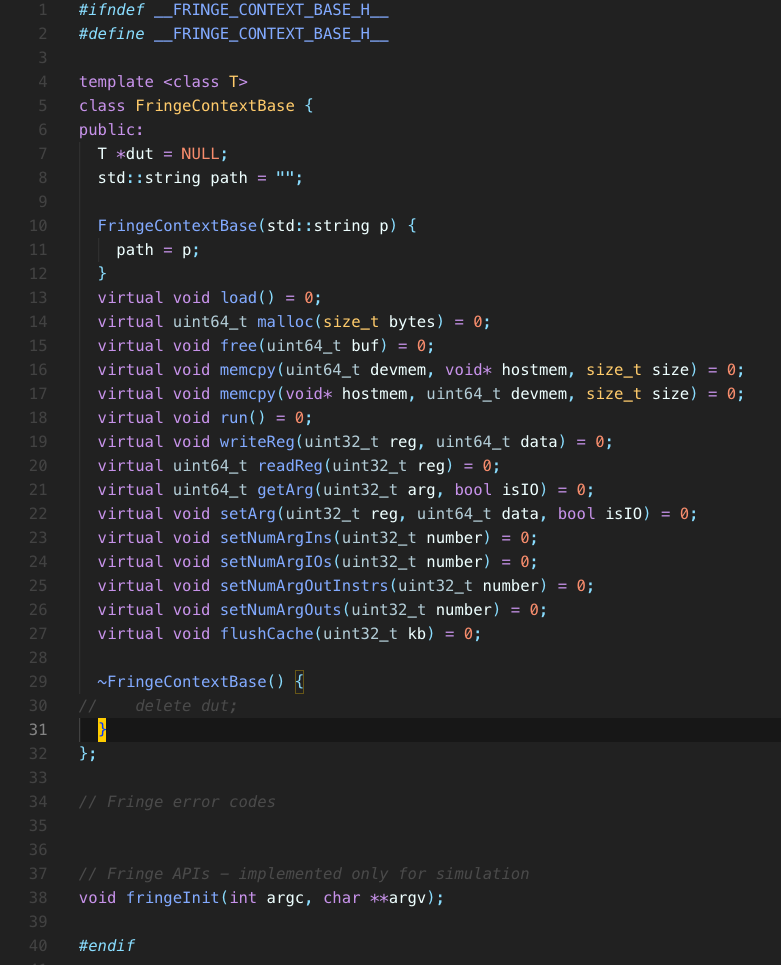
\includegraphics[scale=0.45]{fringecontext.png}
    \caption{FringeContextBase.h}
    \label{fig:fringecontextbase}
    \end{figure}
    
    Table \ref{API} provides a specifications on what each function does.
    For a detailed example, check $fringeArria10/FringeContextArria10.h$.
    Figure \ref{fig:fringecontextbase} shows the complete API.
    
    \begin{table}[t]
    \centering
    \scriptsize
    \begin{tabular}{ll}
       $void$ load() & Loads a bitstream to $Accel$. \\
       $uint64\_t$ malloc($size\_t$ bytes) & Allocates $bytes$ memory. \\
       $void$ free($uint64\_t$ buf) & Free the memory pointer $buf$. \\
       $void$ memcpy($uint64\_t$ devmem, $void\*$ hostmem, $size\_t$ size) & $Accel$ side memcpy. \\ 
       & Memcpy data of $size$ from $devmem$ \\
       & to a virtual address at $host$. \\
       $void$ memcpy($void\*$ hostmem, $uint64\_t$ devmem, $size\_t$ size) & $Host$ side memcpy. \\
       & Memcpy data of $size$ from $hostmem$ \\
       & to a physcial address at $devmem$. \\
       $void$ writeReg($uint32\_t$ reg, $uint64\_t$ data) & Write $data$ to the register located at $reg$ \\
       & starting from the scalar offset. \\
       $uint64\_t$ readReg($uint32\_t$ reg) & Read data stored at the register located at $reg$ \\
       & starting from the scalar offset.
    \end{tabular}
      \caption{Specifications for $Host$ Functions}
      \label{API}
    \end{table}
    
    After implementing these functions, you can generate an executable for the $Host$ code and try to use it to control the execution of $Accel$.
    If the flow works, you will need to update the templates for $Host$ and $Accel$ generation.
    The $Host$ templates are stored at:
    \begin{lstlisting}[language=bash]
    $SPATIAL_HOME/spatial/core/resources/cppgen/fringeArria10/
    \end{lstlisting}
    
    The $Accel$ templates are stored at:
    \begin{lstlisting}[language=bash]
    $SPATIAL_HOME/spatial/core/resources/chiselgen/ \
        template-level/fringeArria10/build/
    \end{lstlisting}
    
    Then, you will need to update the project resources by running:
    \begin{lstlisting}[language=bash]
    cd $SPATIAL_HOME
    bash bin/update_resources.sh
    \end{lstlisting}
    
    You will also need to update the $Makefile$ with your build flow. The $Makefile$ is at
    \begin{lstlisting}[language=bash]
    $SPATIAL_HOME/spatial/core/resources/chiselgen/app-level/Makefile
    \end{lstlisting}
    
    \section{OPAE Implementation}
    \subsection{$Host$}
    The OPAE flow on the $Host$ side can be decoupled into the following stage.
    Each stage can be implemented in a $FringeContext$ function as specified in Table \ref{API}.
    \begin{itemize}
        \item Discover / Search AFU.
            This stage should be implemented in the constructor of $FringeContextArria10$ class.
        \item Acquire ownership of an AFU.
            This stage should be implemented in the constructor of $FringeContextArria10$ class.
        \item Map AFU registers to user space.
            This stage should be implemented in the constructor of $FringeContextArria10$ class.
        \item Allocate / Define shared memory Space.
            This stage should be implemented in the constructor of $FringeContextArria10$ class.
        \item Start / Stop computation on AFU and wait for results.
            Implement $writeReg$, $readReg$ and $memcpy$ functions in $FringeContextArria10$.
            Spatial $Host$ will automatically start and stop the communication on AFU.
            More details can be found in the $run$ function defined in $FringeContextArria10$ class.
        \item Deallocated shared memory.
            This stage should be implemented in the $free$ function.
        \item Relinquish ownership of an AFU.
            This stage should be implemented in the deconstructor of $FringeContextArria10$.
    \end{itemize}
    
    \subsection{$Accel$}
    The OPAE AFU side can communicate with the $Host$ through Avalon-MM (for scalar communication) and 
    AXI4-MM (for DRAM communication).
    The system diagram is shown in Figure \ref{fig:sys}.
    The $Accel$ IP is instantiated as $Top_1$.
    You can connect $io\_M\_AXI\_0$ to $EMIF$ via Avalon-MM and $io\_S\_AVALON\_0$ to the CCI-P bus. 
    The Platform Designer will translate the protocol automatically once you make the connection.
    
    \begin{figure}
    \centering
    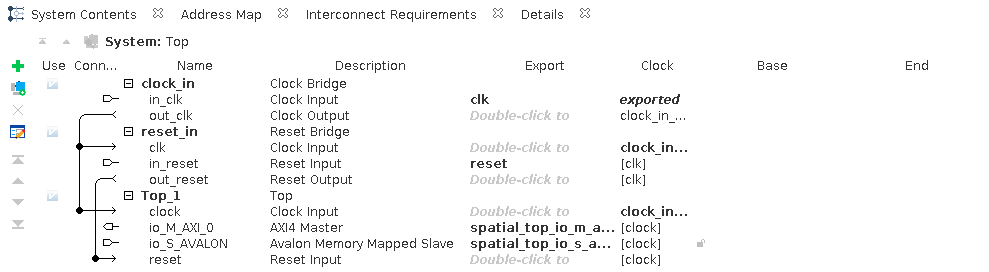
\includegraphics[scale=0.45]{accel.png}
    \caption{Example System Diagram in Platform Designer}
    \label{fig:sys}
    \end{figure}
    
    \end{document}
    